% ------------------------------------------------------------------------
%  create_markers speedup: original per-quadrant ray casting vs. the bulk ray
%  collection optimization (ensure_ray + single bulk cast/distribute pass,
%  see Section~\ref{sec:implementation-host-side-create-markers}).
%  6VYB, local system (test1).
%  Hand-authored from 3 repeated wall-clock timings each, given directly by
%  the user (ms), converted to seconds below:
%      before: 55289.2, 55479.1, 56593.9 ms  ->  55.2892, 55.4791, 56.5939 s
%      after:  33372.2, 33372.2, 33505.0 ms  ->  33.3722, 33.3722, 33.5050 s
%  NOT from test1/bench_runs.csv (t_element_markers) -- that column reflects
%  the already-optimized code on the current branch, so it cannot supply the
%  "before" numbers. Capture method/commit for the "before" run is otherwise
%  unrecorded; flagging this in case the exact figures need to be reproduced
%  later.
%  Bar height = median of the 3 runs; whiskers = min/max. Speedup below is
%  computed on the medians: 55.4791 / 33.3722 = 1.66x.
%  Include with % ------------------------------------------------------------------------
%  create_markers speedup: original per-quadrant ray casting vs. the bulk ray
%  collection optimization (ensure_ray + single bulk cast/distribute pass,
%  see Section~\ref{sec:implementation-host-side-create-markers}).
%  6VYB, local system (test1).
%  Hand-authored from 3 repeated wall-clock timings each, given directly by
%  the user (ms), converted to seconds below:
%      before: 55289.2, 55479.1, 56593.9 ms  ->  55.2892, 55.4791, 56.5939 s
%      after:  33372.2, 33372.2, 33505.0 ms  ->  33.3722, 33.3722, 33.5050 s
%  NOT from test1/bench_runs.csv (t_element_markers) -- that column reflects
%  the already-optimized code on the current branch, so it cannot supply the
%  "before" numbers. Capture method/commit for the "before" run is otherwise
%  unrecorded; flagging this in case the exact figures need to be reproduced
%  later.
%  Bar height = median of the 3 runs; whiskers = min/max. Speedup below is
%  computed on the medians: 55.4791 / 33.3722 = 1.66x.
%  Include with % ------------------------------------------------------------------------
%  create_markers speedup: original per-quadrant ray casting vs. the bulk ray
%  collection optimization (ensure_ray + single bulk cast/distribute pass,
%  see Section~\ref{sec:implementation-host-side-create-markers}).
%  6VYB, local system (test1).
%  Hand-authored from 3 repeated wall-clock timings each, given directly by
%  the user (ms), converted to seconds below:
%      before: 55289.2, 55479.1, 56593.9 ms  ->  55.2892, 55.4791, 56.5939 s
%      after:  33372.2, 33372.2, 33505.0 ms  ->  33.3722, 33.3722, 33.5050 s
%  NOT from test1/bench_runs.csv (t_element_markers) -- that column reflects
%  the already-optimized code on the current branch, so it cannot supply the
%  "before" numbers. Capture method/commit for the "before" run is otherwise
%  unrecorded; flagging this in case the exact figures need to be reproduced
%  later.
%  Bar height = median of the 3 runs; whiskers = min/max. Speedup below is
%  computed on the medians: 55.4791 / 33.3722 = 1.66x.
%  Include with % ------------------------------------------------------------------------
%  create_markers speedup: original per-quadrant ray casting vs. the bulk ray
%  collection optimization (ensure_ray + single bulk cast/distribute pass,
%  see Section~\ref{sec:implementation-host-side-create-markers}).
%  6VYB, local system (test1).
%  Hand-authored from 3 repeated wall-clock timings each, given directly by
%  the user (ms), converted to seconds below:
%      before: 55289.2, 55479.1, 56593.9 ms  ->  55.2892, 55.4791, 56.5939 s
%      after:  33372.2, 33372.2, 33505.0 ms  ->  33.3722, 33.3722, 33.5050 s
%  NOT from test1/bench_runs.csv (t_element_markers) -- that column reflects
%  the already-optimized code on the current branch, so it cannot supply the
%  "before" numbers. Capture method/commit for the "before" run is otherwise
%  unrecorded; flagging this in case the exact figures need to be reproduced
%  later.
%  Bar height = median of the 3 runs; whiskers = min/max. Speedup below is
%  computed on the medians: 55.4791 / 33.3722 = 1.66x.
%  Include with \input{figures/create_markers_speedup}
%  Needs \usepackage{pgfplots} in the preamble.
% ------------------------------------------------------------------------
\pgfplotsset{compat=1.16}

\definecolor{cmbefore}{HTML}{D95F02}
\definecolor{cmafter}{HTML}{2C5F8D}

\begin{figure}[!htb]
\centering
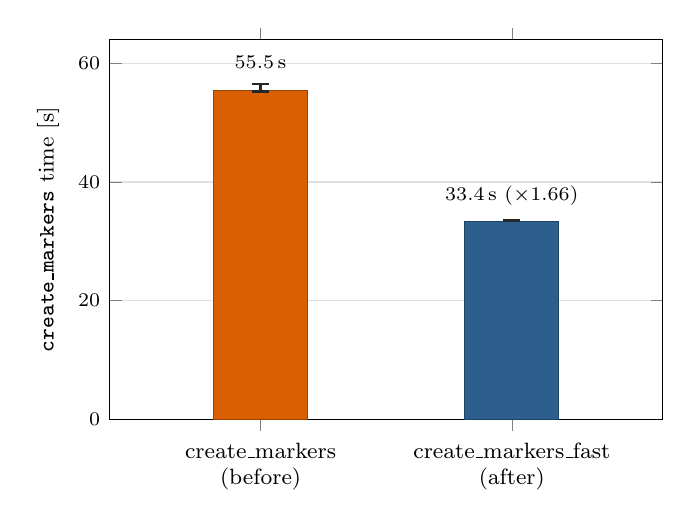
\begin{tikzpicture}
\begin{axis}[
    ybar,
    width=8.6cm, height=6.4cm,
    bar width=34pt,
    xmin=-0.6, xmax=1.6,
    xtick={0,1},
    xticklabels={\snakecase{create\_markers}\\(before),\snakecase{create\_markers\_fast}\\(after)},
    xticklabel style={font=\footnotesize, align=center, yshift=-0.2ex},
    ymin=0, ymax=64,
    ylabel={\texttt{create\_markers} time [s]},
    ylabel style={font=\footnotesize},
    tick label style={font=\scriptsize},
    ymajorgrids=true,
    major grid style={black!12},
    error bars/error bar style={black!85, line width=0.8pt},
    error bars/error mark options={
      mark size=3pt, rotate=90, line width=0.8pt, black!85,
    },
]
  \addplot+[
    ybar, bar shift=0pt, fill=cmbefore, draw=cmbefore!70!black, line width=0.4pt,
    error bars/.cd, y dir=both, y explicit,
  ] table[row sep=\\, x=x, y=y, y error plus=ep, y error minus=em] {
    x y ep em \\
    0 55.4791 1.1148 0.1899 \\
  };
  \addplot+[
    ybar, bar shift=0pt, fill=cmafter, draw=cmafter!70!black, line width=0.4pt,
    error bars/.cd, y dir=both, y explicit,
  ] table[row sep=\\, x=x, y=y, y error plus=ep, y error minus=em] {
    x y ep em \\
    1 33.3722 0.1328 0.0000 \\
  };

  % One label per bar, above the whisker cap: median value, and (for "after")
  % the speedup relative to "before" -- kept as a single node per bar rather
  % than two stacked ones, since the whisker span is only ~1s/~0.1s against a
  % 0-64s axis and two separately-anchored nodes there collide.
  \node[font=\scriptsize, anchor=south, yshift=2pt]
    at (axis cs:0,56.5939) {55.5\,s};
  \node[font=\scriptsize, anchor=south, yshift=2pt]
    at (axis cs:1,33.5050) {33.4\,s ($\times$1.66)};
\end{axis}
\end{tikzpicture}

\caption[\texttt{create\_markers} speedup from bulk ray collection]{\textbf{\snakecase{create\_markers} vs.\ \snakecase{create\_markers\_fast} wall time, 6VYB (test1).} Median over 3 runs, whiskers spanning fastest to slowest; the label above each bar is that median in seconds, with the speedup relative to \snakecase{create\_markers} in parentheses. \snakecase{create\_markers\_fast} collects all needed rays first with \snakecase{ensure\_ray}, then casts and distributes them in one bulk pass before classification (Section~\ref{sec:implementation-host-side-create-markers}). Measured on the local system (Table~\ref{tab:test-systems}).}
\label{fig:create-markers-speedup}
\end{figure}

%  Needs \usepackage{pgfplots} in the preamble.
% ------------------------------------------------------------------------
\pgfplotsset{compat=1.16}

\definecolor{cmbefore}{HTML}{D95F02}
\definecolor{cmafter}{HTML}{2C5F8D}

\begin{figure}[!htb]
\centering
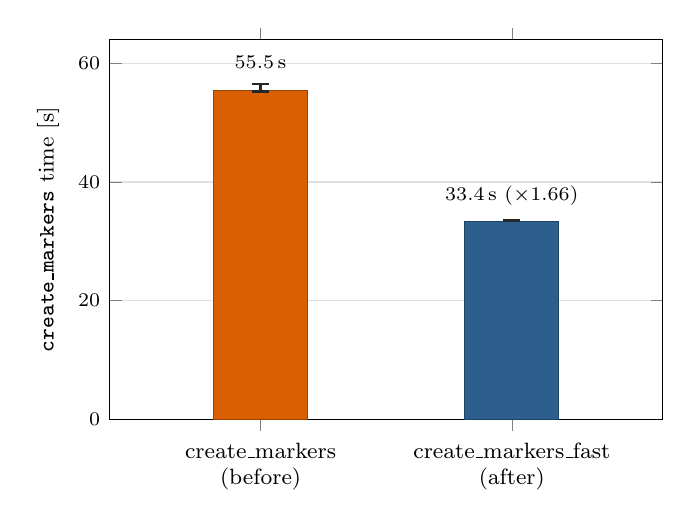
\begin{tikzpicture}
\begin{axis}[
    ybar,
    width=8.6cm, height=6.4cm,
    bar width=34pt,
    xmin=-0.6, xmax=1.6,
    xtick={0,1},
    xticklabels={\snakecase{create\_markers}\\(before),\snakecase{create\_markers\_fast}\\(after)},
    xticklabel style={font=\footnotesize, align=center, yshift=-0.2ex},
    ymin=0, ymax=64,
    ylabel={\texttt{create\_markers} time [s]},
    ylabel style={font=\footnotesize},
    tick label style={font=\scriptsize},
    ymajorgrids=true,
    major grid style={black!12},
    error bars/error bar style={black!85, line width=0.8pt},
    error bars/error mark options={
      mark size=3pt, rotate=90, line width=0.8pt, black!85,
    },
]
  \addplot+[
    ybar, bar shift=0pt, fill=cmbefore, draw=cmbefore!70!black, line width=0.4pt,
    error bars/.cd, y dir=both, y explicit,
  ] table[row sep=\\, x=x, y=y, y error plus=ep, y error minus=em] {
    x y ep em \\
    0 55.4791 1.1148 0.1899 \\
  };
  \addplot+[
    ybar, bar shift=0pt, fill=cmafter, draw=cmafter!70!black, line width=0.4pt,
    error bars/.cd, y dir=both, y explicit,
  ] table[row sep=\\, x=x, y=y, y error plus=ep, y error minus=em] {
    x y ep em \\
    1 33.3722 0.1328 0.0000 \\
  };

  % One label per bar, above the whisker cap: median value, and (for "after")
  % the speedup relative to "before" -- kept as a single node per bar rather
  % than two stacked ones, since the whisker span is only ~1s/~0.1s against a
  % 0-64s axis and two separately-anchored nodes there collide.
  \node[font=\scriptsize, anchor=south, yshift=2pt]
    at (axis cs:0,56.5939) {55.5\,s};
  \node[font=\scriptsize, anchor=south, yshift=2pt]
    at (axis cs:1,33.5050) {33.4\,s ($\times$1.66)};
\end{axis}
\end{tikzpicture}

\caption[\texttt{create\_markers} speedup from bulk ray collection]{\textbf{\snakecase{create\_markers} vs.\ \snakecase{create\_markers\_fast} wall time, 6VYB (test1).} Median over 3 runs, whiskers spanning fastest to slowest; the label above each bar is that median in seconds, with the speedup relative to \snakecase{create\_markers} in parentheses. \snakecase{create\_markers\_fast} collects all needed rays first with \snakecase{ensure\_ray}, then casts and distributes them in one bulk pass before classification (Section~\ref{sec:implementation-host-side-create-markers}). Measured on the local system (Table~\ref{tab:test-systems}).}
\label{fig:create-markers-speedup}
\end{figure}

%  Needs \usepackage{pgfplots} in the preamble.
% ------------------------------------------------------------------------
\pgfplotsset{compat=1.16}

\definecolor{cmbefore}{HTML}{D95F02}
\definecolor{cmafter}{HTML}{2C5F8D}

\begin{figure}[!htb]
\centering
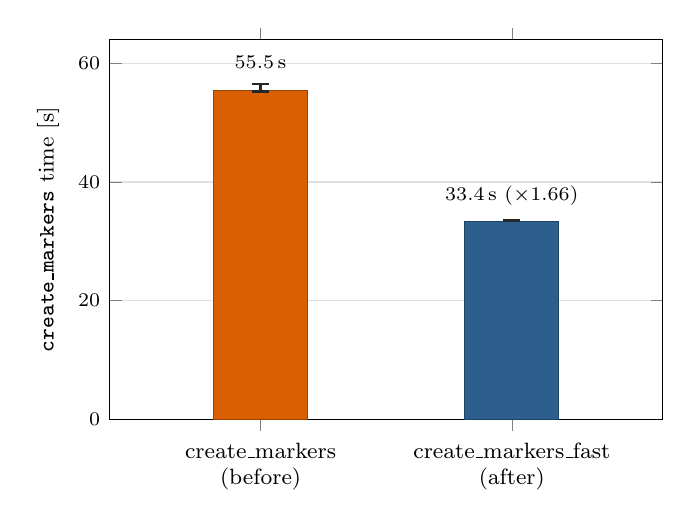
\begin{tikzpicture}
\begin{axis}[
    ybar,
    width=8.6cm, height=6.4cm,
    bar width=34pt,
    xmin=-0.6, xmax=1.6,
    xtick={0,1},
    xticklabels={\snakecase{create\_markers}\\(before),\snakecase{create\_markers\_fast}\\(after)},
    xticklabel style={font=\footnotesize, align=center, yshift=-0.2ex},
    ymin=0, ymax=64,
    ylabel={\texttt{create\_markers} time [s]},
    ylabel style={font=\footnotesize},
    tick label style={font=\scriptsize},
    ymajorgrids=true,
    major grid style={black!12},
    error bars/error bar style={black!85, line width=0.8pt},
    error bars/error mark options={
      mark size=3pt, rotate=90, line width=0.8pt, black!85,
    },
]
  \addplot+[
    ybar, bar shift=0pt, fill=cmbefore, draw=cmbefore!70!black, line width=0.4pt,
    error bars/.cd, y dir=both, y explicit,
  ] table[row sep=\\, x=x, y=y, y error plus=ep, y error minus=em] {
    x y ep em \\
    0 55.4791 1.1148 0.1899 \\
  };
  \addplot+[
    ybar, bar shift=0pt, fill=cmafter, draw=cmafter!70!black, line width=0.4pt,
    error bars/.cd, y dir=both, y explicit,
  ] table[row sep=\\, x=x, y=y, y error plus=ep, y error minus=em] {
    x y ep em \\
    1 33.3722 0.1328 0.0000 \\
  };

  % One label per bar, above the whisker cap: median value, and (for "after")
  % the speedup relative to "before" -- kept as a single node per bar rather
  % than two stacked ones, since the whisker span is only ~1s/~0.1s against a
  % 0-64s axis and two separately-anchored nodes there collide.
  \node[font=\scriptsize, anchor=south, yshift=2pt]
    at (axis cs:0,56.5939) {55.5\,s};
  \node[font=\scriptsize, anchor=south, yshift=2pt]
    at (axis cs:1,33.5050) {33.4\,s ($\times$1.66)};
\end{axis}
\end{tikzpicture}

\caption[\texttt{create\_markers} speedup from bulk ray collection]{\textbf{\snakecase{create\_markers} vs.\ \snakecase{create\_markers\_fast} wall time, 6VYB (test1).} Median over 3 runs, whiskers spanning fastest to slowest; the label above each bar is that median in seconds, with the speedup relative to \snakecase{create\_markers} in parentheses. \snakecase{create\_markers\_fast} collects all needed rays first with \snakecase{ensure\_ray}, then casts and distributes them in one bulk pass before classification (Section~\ref{sec:implementation-host-side-create-markers}). Measured on the local system (Table~\ref{tab:test-systems}).}
\label{fig:create-markers-speedup}
\end{figure}

%  Needs \usepackage{pgfplots} in the preamble.
% ------------------------------------------------------------------------
\pgfplotsset{compat=1.16}

\definecolor{cmbefore}{HTML}{D95F02}
\definecolor{cmafter}{HTML}{2C5F8D}

\begin{figure}[!htb]
\centering
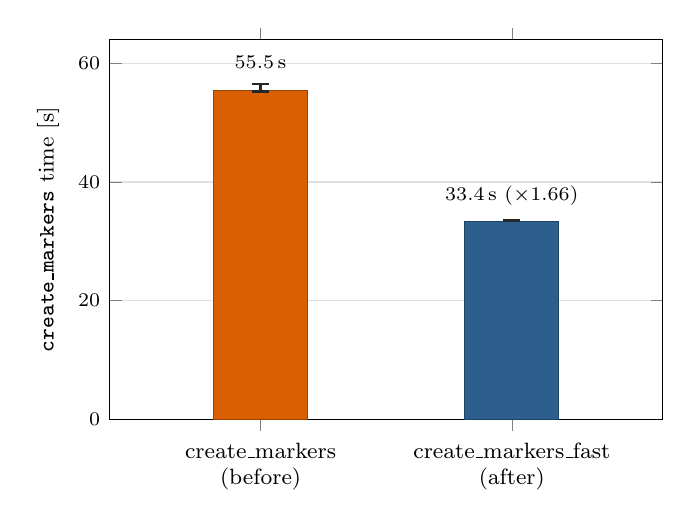
\begin{tikzpicture}
\begin{axis}[
    ybar,
    width=8.6cm, height=6.4cm,
    bar width=34pt,
    xmin=-0.6, xmax=1.6,
    xtick={0,1},
    xticklabels={\snakecase{create\_markers}\\(before),\snakecase{create\_markers\_fast}\\(after)},
    xticklabel style={font=\footnotesize, align=center, yshift=-0.2ex},
    ymin=0, ymax=64,
    ylabel={\texttt{create\_markers} time [s]},
    ylabel style={font=\footnotesize},
    tick label style={font=\scriptsize},
    ymajorgrids=true,
    major grid style={black!12},
    error bars/error bar style={black!85, line width=0.8pt},
    error bars/error mark options={
      mark size=3pt, rotate=90, line width=0.8pt, black!85,
    },
]
  \addplot+[
    ybar, bar shift=0pt, fill=cmbefore, draw=cmbefore!70!black, line width=0.4pt,
    error bars/.cd, y dir=both, y explicit,
  ] table[row sep=\\, x=x, y=y, y error plus=ep, y error minus=em] {
    x y ep em \\
    0 55.4791 1.1148 0.1899 \\
  };
  \addplot+[
    ybar, bar shift=0pt, fill=cmafter, draw=cmafter!70!black, line width=0.4pt,
    error bars/.cd, y dir=both, y explicit,
  ] table[row sep=\\, x=x, y=y, y error plus=ep, y error minus=em] {
    x y ep em \\
    1 33.3722 0.1328 0.0000 \\
  };

  % One label per bar, above the whisker cap: median value, and (for "after")
  % the speedup relative to "before" -- kept as a single node per bar rather
  % than two stacked ones, since the whisker span is only ~1s/~0.1s against a
  % 0-64s axis and two separately-anchored nodes there collide.
  \node[font=\scriptsize, anchor=south, yshift=2pt]
    at (axis cs:0,56.5939) {55.5\,s};
  \node[font=\scriptsize, anchor=south, yshift=2pt]
    at (axis cs:1,33.5050) {33.4\,s ($\times$1.66)};
\end{axis}
\end{tikzpicture}

\caption[\texttt{create\_markers} speedup from bulk ray collection]{\textbf{\snakecase{create\_markers} vs.\ \snakecase{create\_markers\_fast} wall time, 6VYB (test1).} Median over 3 runs, whiskers spanning fastest to slowest; the label above each bar is that median in seconds, with the speedup relative to \snakecase{create\_markers} in parentheses. \snakecase{create\_markers\_fast} collects all needed rays first with \snakecase{ensure\_ray}, then casts and distributes them in one bulk pass before classification (Section~\ref{sec:implementation-host-side-create-markers}). Measured on the local system (Table~\ref{tab:test-systems}).}
\label{fig:create-markers-speedup}
\end{figure}
